% !TeX root = RJwrapper.tex
\title{HUMANS AND DOMICILE TYPE - A COMMUNITY ECOLOGY APPROACH}
\author{by Ann Wozniak AIA, NCARB, LEED AP BD+C, and NCIDQ}

\maketitle

\abstract{%
Life history theory suggests that there are fitness trade-offs between
survival and reproduction when an individual is exposed to environmental
stress. Stress present in both physical and social environments can
trigger physiological, behavioral, and developmental responses in an
individual, impacting their health. Research has also shown that the
lack of social connectedness has a negative impact on health. In this
independent analysis of data from the European Social Survey European
Research Infrastructure Consortium (ESS ERIC), a cross-national
longitudinal survey from 2002-2018 that included over thirty (30)
countries in Europe (n=106,320) suggests that domicile type may be used
as a predictor of health. Stressors such as being a victim of burglary
or assault, living with a partner, being divorced, having a parent that
is absent or deceased, or having a mother that is self-employed tend to
have poorer health outcomes. Social involvement in the community through
voting has a significant effect on positive health outcomes. Data from
the study also suggest that respondents' perceptions of safety and
happiness may act as a proximate mechanism with a significant effect on
health outcomes. The data has been adapted to fit a human community
framework to better understand if health outcomes may be predicted at a
community level. Linking social connectedness to the physical
environment will allow researchers, architects, and policy makers to
better understand the important relationship between these social
dimensions in the built environment and health outcomes.
}

\hypertarget{introduction}{%
\subsection{Introduction}\label{introduction}}

Arguably, the human species could be the most important driver of
ecological communities on the planet, with human behavior attributed to
major climate change. Not only are humans driving the next mass
extinctions in the Anthropocene, according to \citet{Tilman}, they are
changing the identities and diversity in communities. If age, gender,
and spatial distributions are common factors analyzed in community and
population ecology, why has there been less work on human communities
\citep{McKenzie}? Defining populations by age and gender is a common
practice in community ecology that can easily be applied to humans,
treating our societies as ecological communities. \citet{Dreiss} used a
similar method in defining lizard populations to examine sexual
selection. \citet{Polis} found that the functional differences of
feeding patterns between age and gender is significant enough to
represent different ``ecological species.'' This study will synthesize
data from a longitudinal study to define ``species'' within a human
community framework where age and gender determine species.

Examining health through an ecological lens in context of spatial
distribution, social connections, and perception measured as happiness
has been studied to a lesser degree. \citet{Winterton} found that
diversity within a community can impact health outcomes. It has been
found that functional diversity among the plant community can produce
higher abundance and biomass \citep{Tilman}. From these studies, one
might expect environmental variables to be significantly correlated to
each other, with domicile type positively related to health, happiness,
and social connectedness. Diversity across sites
(country-by-domicile-type) is expected to be significantly and
positively correlated to all of the environmental variables: domicile
type, country, happiness, health, and social connectedness.
\citet{Planchuelo} has found that cities are rich in biodiversity, and
likely in different ages and types of people as well. As such, it is
expected that Shannon diversity and effective number of species will be
highest in cities. Using community ecology methods and analysis, site
and species will be measured for diversity while environmental data will
be analyzed within and across sites.

This study takes a deeper dive into existing data to better understand
the correlations and linear relationships, using a community ecology
framework where country-by-domicile-type are sites and age-by-gender are
``species''. Domicile type is broken into five categories: a big city, a
country or village, a farm or home in the countryside, the suburbs or
outskirts of a big city and a town or small city. Thirty-eight countries
were included in this analysis, including Albania, Austria, Belgium,
Bulgaria, Croatia, Cyprus, Czechia, Denmark, Estonia, Finland, France,
Germany, Greece, Hungary, Iceland, Ireland, Israel, Italy, Kosovo,
Latvia, Lithuania, Luxembourg, Montenegro, Netherlands, Norway, Poland,
Portugal, Romania, Russian Federation, Serbia, Slovakia, Slovenia,
Spain, Sweden, Switzerland, Turkey, Ukraine, and the United Kingdom.
This analysis will analyze site and ``species'' as well as environmental
data such as health, happiness, and social connectedness related to
country and domicile type through a community ecology framework.

\hypertarget{methods}{%
\subsection{Methods}\label{methods}}

My project methodology analyzed existing data from the European Social
Survey European Research Infrastructure Consortium (ESS ERIC), a
cross-national longitudinal survey from 2002-2018 that included over
thirty (30) countries in Europe (n=106,320). This particular study was
unique to my area of research in that it included information on
domicile type, health, quality of life, and questions about social
connectedness. In addition, the data was accessible free of charge,
relatively unrestricted for further analysis and interpretation by
researchers as well as provided a multi-year database, spanning more
than a decade of responses. This information is critical in setting the
groundwork for my own research, which may indicate a temporal permanence
trend in the relationship between domicile type, social connectedness
and perception to health outcomes.

Surveys were conducted every two years, separated into nine data sets.
They were downloaded from the European Social Survey website at
\url{https://www.europeansocialsurvey.org/data/round-index.html}. The
following data fields were extracted from each survey and compiled
together in Table 1.

\begin{Schunk}

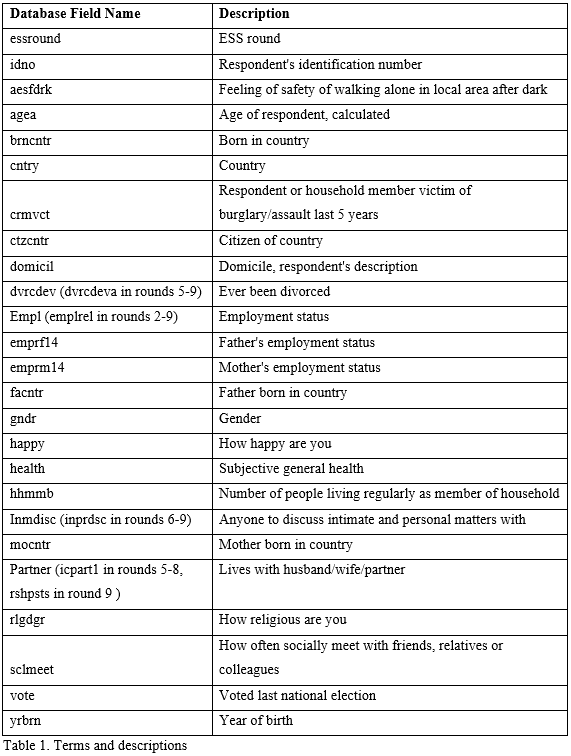
\includegraphics[width=1\linewidth]{C:/Users/annwozniak/Desktop/EEB_Final_Project_Wozniak/Figures/Terms_and_descriptions} \end{Schunk}

Before merging the surveys, I had to recode two variables. Where the
field description ``anyone to discuss intimate and personal matters
with'' (inprdsc) was used in rounds six through nine, 0 indicated ``no''
and 1-6 indicated ``yes'' whereas the same field description (inmdisc)
in the other rounds only had ``yes'' (1) and ``no'' (2). To match, I
recoded the fields in rounds six through nine using 1-6 as ``yes'' (1)
and 0 to ``no'' (2). Where the field description ``lives with
husband/wife/partner'' (rshpsts) was used in round nine, 3-4 indicated
``living with a partner'' whereas 1-2 and 5-6 indicated ``does not live
with a partner''. The same field description ``lives with
husband/wife/partner'' (partner) in rounds one through four, only had
``lives with partner'' (1) or ``does not live with partner'' (2). To
match, I recoded the field in round nine using 3-4 as ``lives with
partner'' (1) and the rest to ``does not live with partner'' (2). All of
the other fields with conflicting field names and same descriptions were
coded the same and simply merged under universal database names as
indicated in Table 1. It was important to maintain consistent coding
before merging surveys to avoid discrepancy in interpretation.

After merging the surveys, additional fields were generated with
categorical variables. Utilizing data from the field describing
``feeling of safety while walking alone in local area after dark''
(aesfdrk), a ``feeling of safety, derived'' (calc\_safe) categorical
field was generated where ``very safe'' or ``safe'' meant ``safe'' (1)
and everything else meant ``not safe'' (0), unless missing. If data was
missing, I derived safety from the original survey question description
``respondent or household member victim of burglary/assault last 5
years'' (crmvct) where responses indicated ``yes,'' they were
categorized as ``not safe'' (0). Where responses indicated a ``no,''
they were categorized as ``safe'' (1). Utilizing data from the original
survey question description ``subjective general health'' (health)
field, a ``Subjective general health'' (calc\_health) categorical field
was generated where ``very good'' or ``good'' health meant ``good
health'' (1) and everything else meant ``bad health'' (0), unless
missing. Creating categorical variations of safety and health made
preliminary logistic regression analysis possible in IBM SPSS Statistics
(SPSS) software, but was not necessary using R.

The merged survey data set required additional clean-up before running
any statistical analyses. Another new field ``household size''
(Calc\_household\_size) was added to simplify the continuour field
``Number of people living regularly as member of household'' (hhmmb)
where anyresponses of seven people or over were categorized to ``seven
and over''. Any cases with missing values were excluded from this study.
Equal distribution across domicile types were randomly selected for each
category including ``big city'', ``suburbs or outskirts of a big city'',
``town or small city'', ``country village'', and ``farm or home in
countryside''. This final data set was where the data and metadata in
this analysis were extracted from.

Since this project applies analyses used in community ecology to the
built environment, the datasets have to be set up as sites and
``species'' and relevant metadata must be compiled. From SPSS, I
exported the data to a comma delimited (csv) file. In Excel, I was able
to combine the country with the domicile type description to generate a
site field. The respondent's age and gender were combined to generate
the species field. A pivot table was used to generate a matrix of the
total number of species in each site. This data was saved as a comma
delimited (csv) file to be imported into R. The metadata was generated
in a very similar fashion where site, country, domicile type, happy,
health, and social (sclmeet) data were exported into a new comma
delimited (csv) file. This time a pivot table was used to derive the
average happy scale, health scale and social scale by each site. That
data was then saved as the metadata comma delimited (csv) file to be
imported into R for analysis. The data is now set up as community
ecology data for analysis in R.

The linear regressions and community ecology diversity methods were used
to answer the questions set out in this paper. I ran multiple linear
regression models to check if domicile type is significantly correlated
to health, happiness or social connectedness. Similarly, I ran multiple
linear regression models to check if happiness or social connectedness
significantly correlated to health. Finally, I analyzed alpha diversity
within each site by calculating species number, Shannon diversity, and
the effective number of species, and effective number of species
(rounded) as well as beta diversity across sites using Bray-Curtis and
Jaccard methods to determine which sites are most similar and
dissimilar.

\hypertarget{data-disclaimer}{%
\subsection{Data Disclaimer}\label{data-disclaimer}}

Some of the data applied in this analysis is based on the ESS Data
Rounds 1-9. The data is provided by
\url{https://www.europeansocialsurvey.org/data/round-index.html} and
prepared and made available by NSD - Norwegian Centre for Research Data.
Neither \url{https://www.europeansocialsurvey.org/data/round-index.html}
nor NSD are responsible for the analyses and/or interpretation of the
data presented in my independent analysis.

\hypertarget{results}{%
\subsection{Results}\label{results}}

Is domicile type significantly correlated to health? When looking at the
relationships among environmental variables, domicile by health (Figure
1), a linear regression analysis and Kruskal-Wallis rank sum test shows
that, overall, domicile type is not significantly correlated to health,
p = 0.4977 and 0.5162 respectively

\begin{Schunk}
\begin{figure}
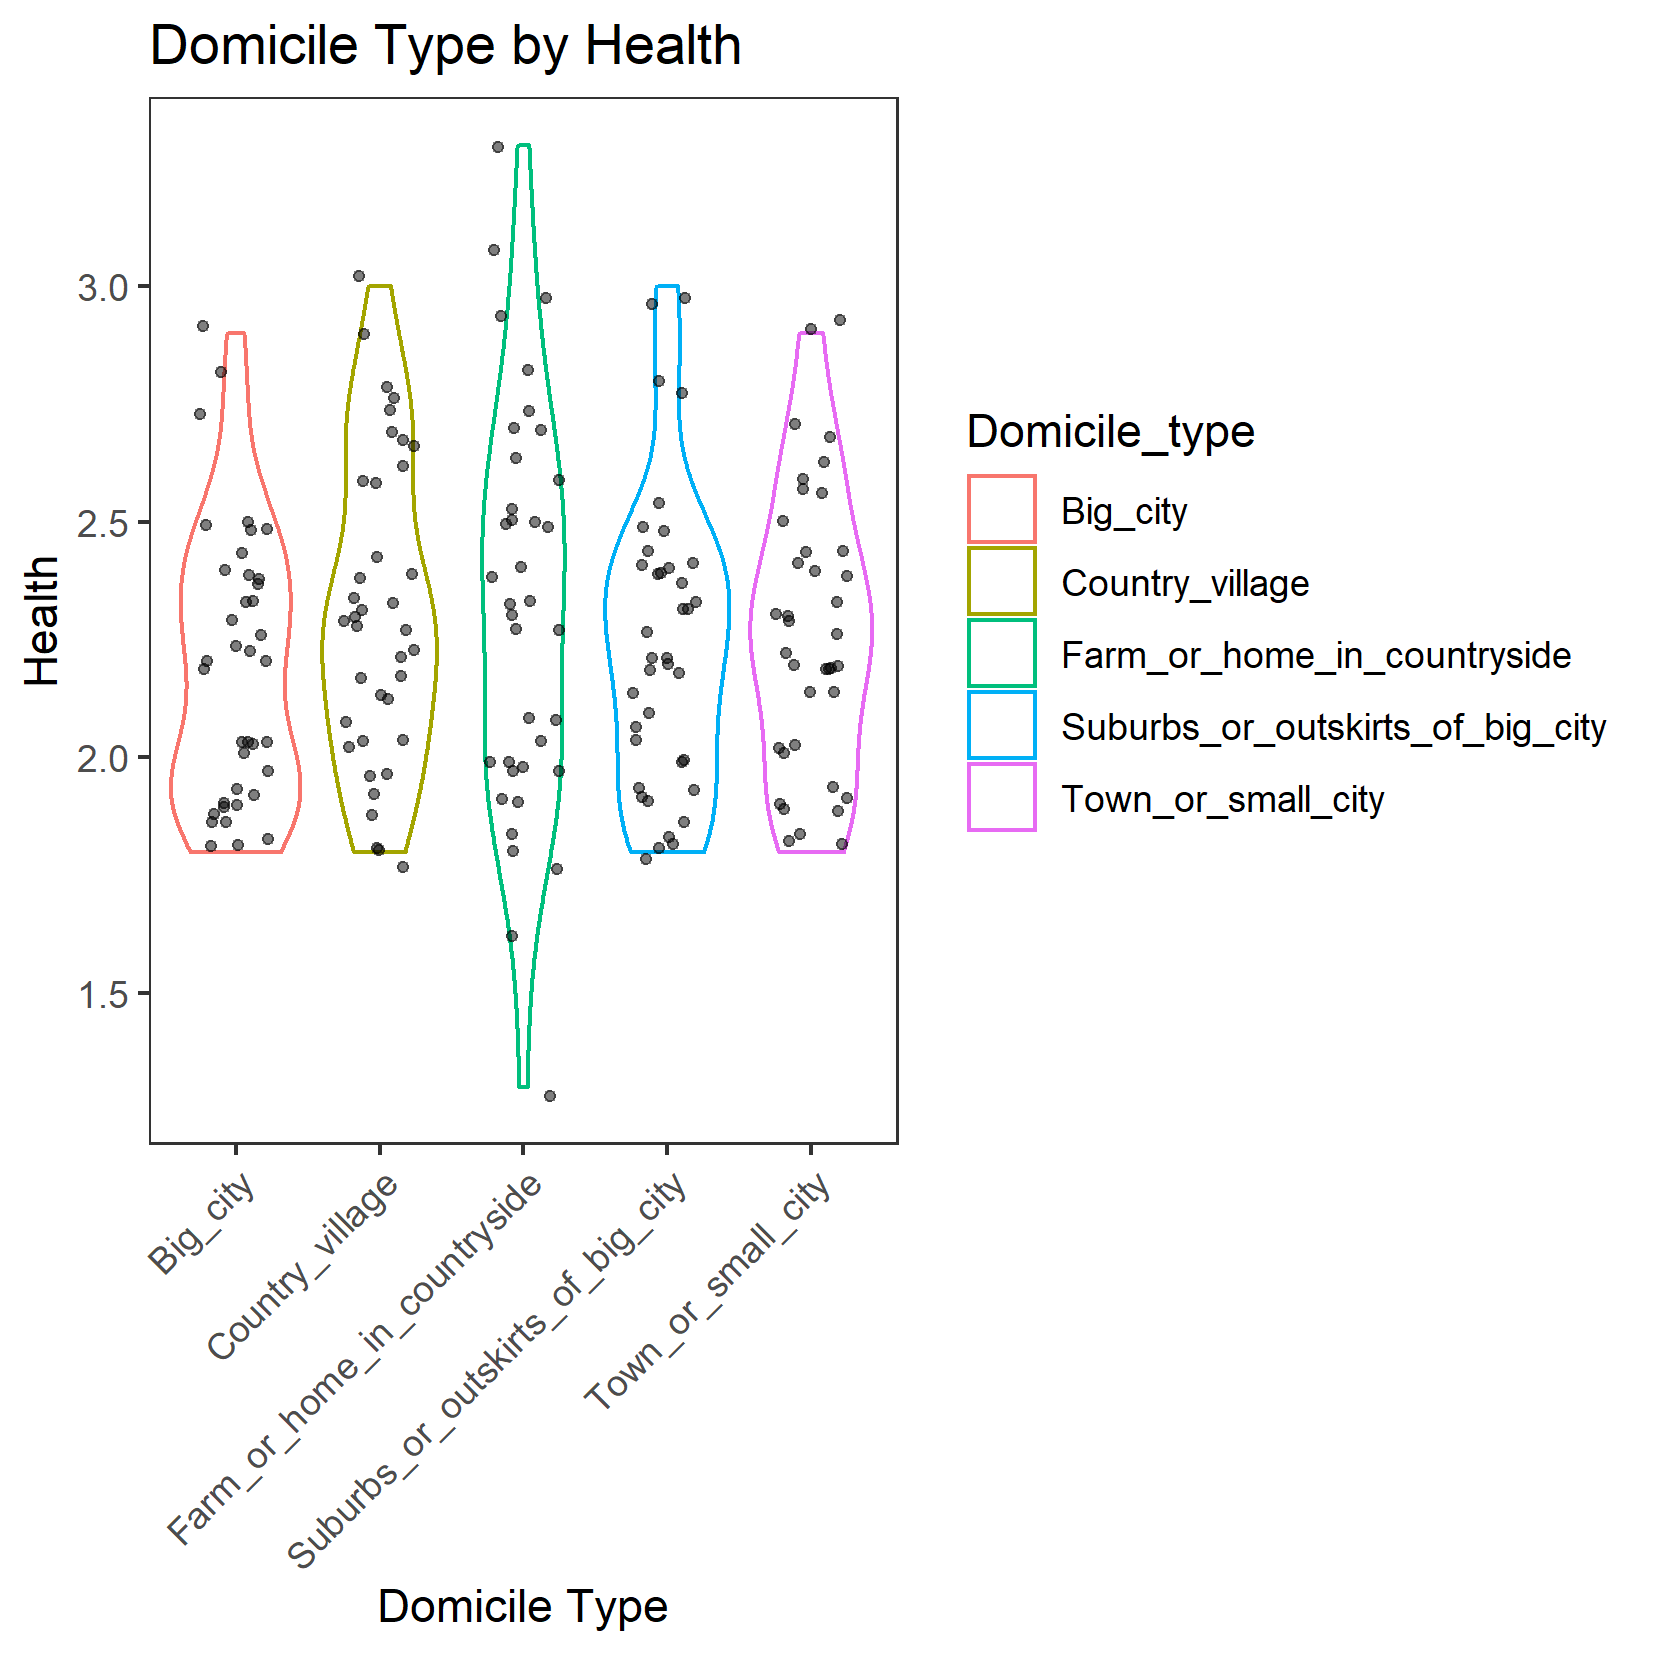
\includegraphics[width=1\linewidth]{C:/Users/annwozniak/Desktop/EEB_Final_Project_Wozniak/Figures/graph_violin_Domicile_by_Health} \caption[Domicile type by health (1-5 scale, good to poor)]{Domicile type by health (1-5 scale, good to poor)}\label{fig:fig.1}
\end{figure}
\end{Schunk}

Is domicile type significantly correlated to happiness? When looking at
the relationships among environmental variables, domicile by happiness
(Fig. 2) , a linear regression analysis and Kruskal-Wallis rank sum test
shows that, overall, domicile type is not significantly correlated to
happiness, p = 0.9117 and 0.9938 respectively.

\begin{Schunk}
\begin{figure}
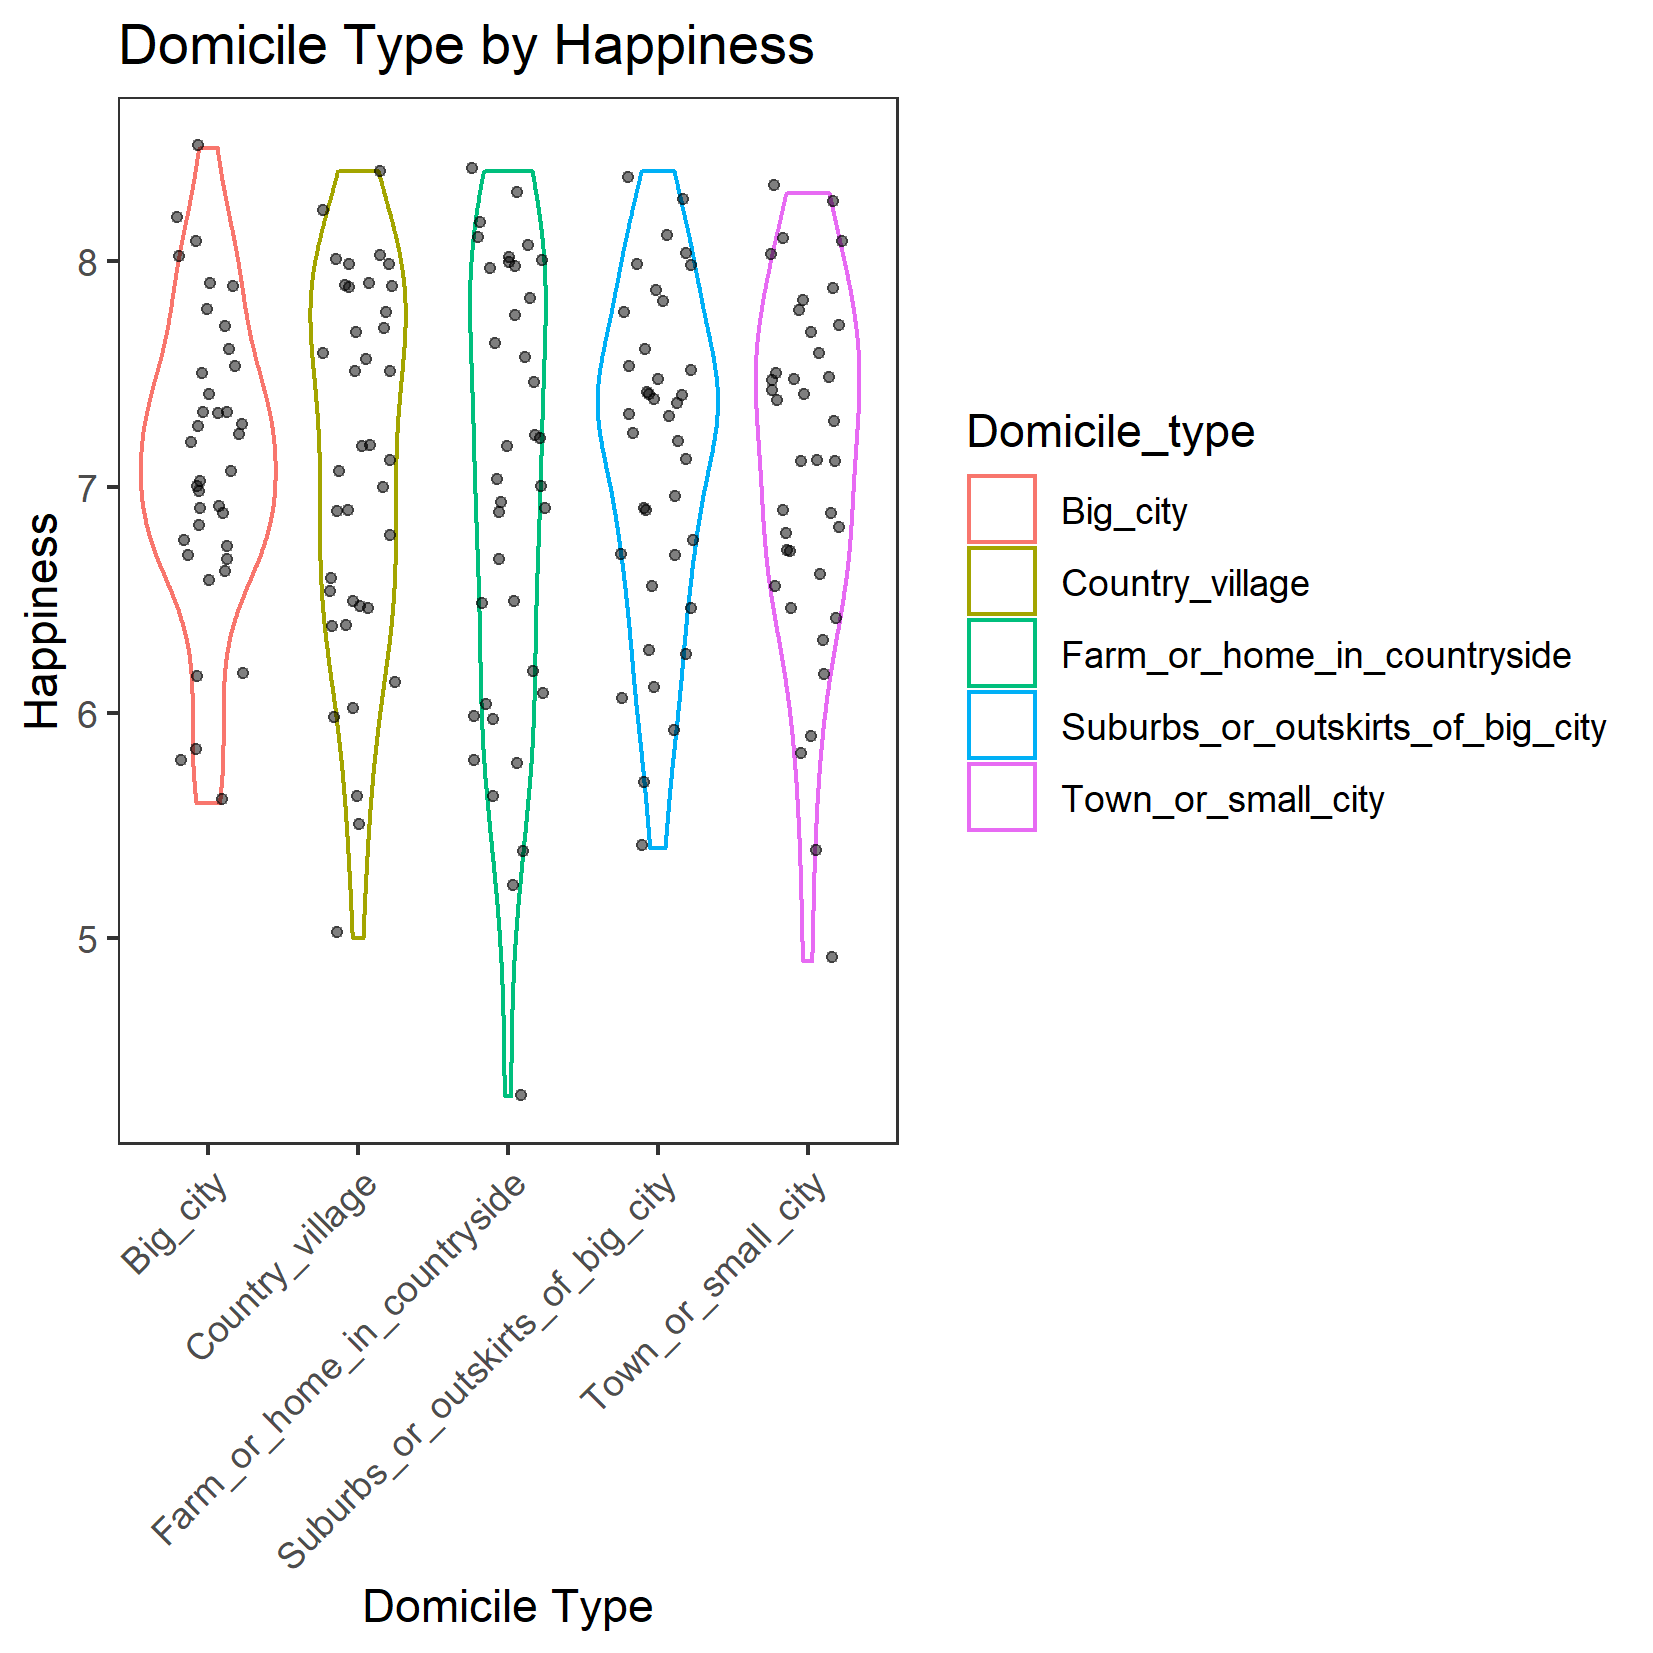
\includegraphics[width=1\linewidth]{C:/Users/annwozniak/Desktop/EEB_Final_Project_Wozniak/Figures/graph_violin_Domicile_by_Happiness} \caption[Domicile type by happiness (0-10 scale, unhappy to happy)]{Domicile type by happiness (0-10 scale, unhappy to happy)}\label{fig:fig.2}
\end{figure}
\end{Schunk}

Is domicile type significantly correlated to social connectedness? When
looking at the relationships among environmental variables, domicile by
social connectedness (Fig. 3), a linear regression analysis and
Kruskal-Wallis rank sum test shows that, overall, domicile type is not
significantly correlated to social connectedness, p = 0.9788 and 0.9193
respectively.

\begin{Schunk}
\begin{figure}
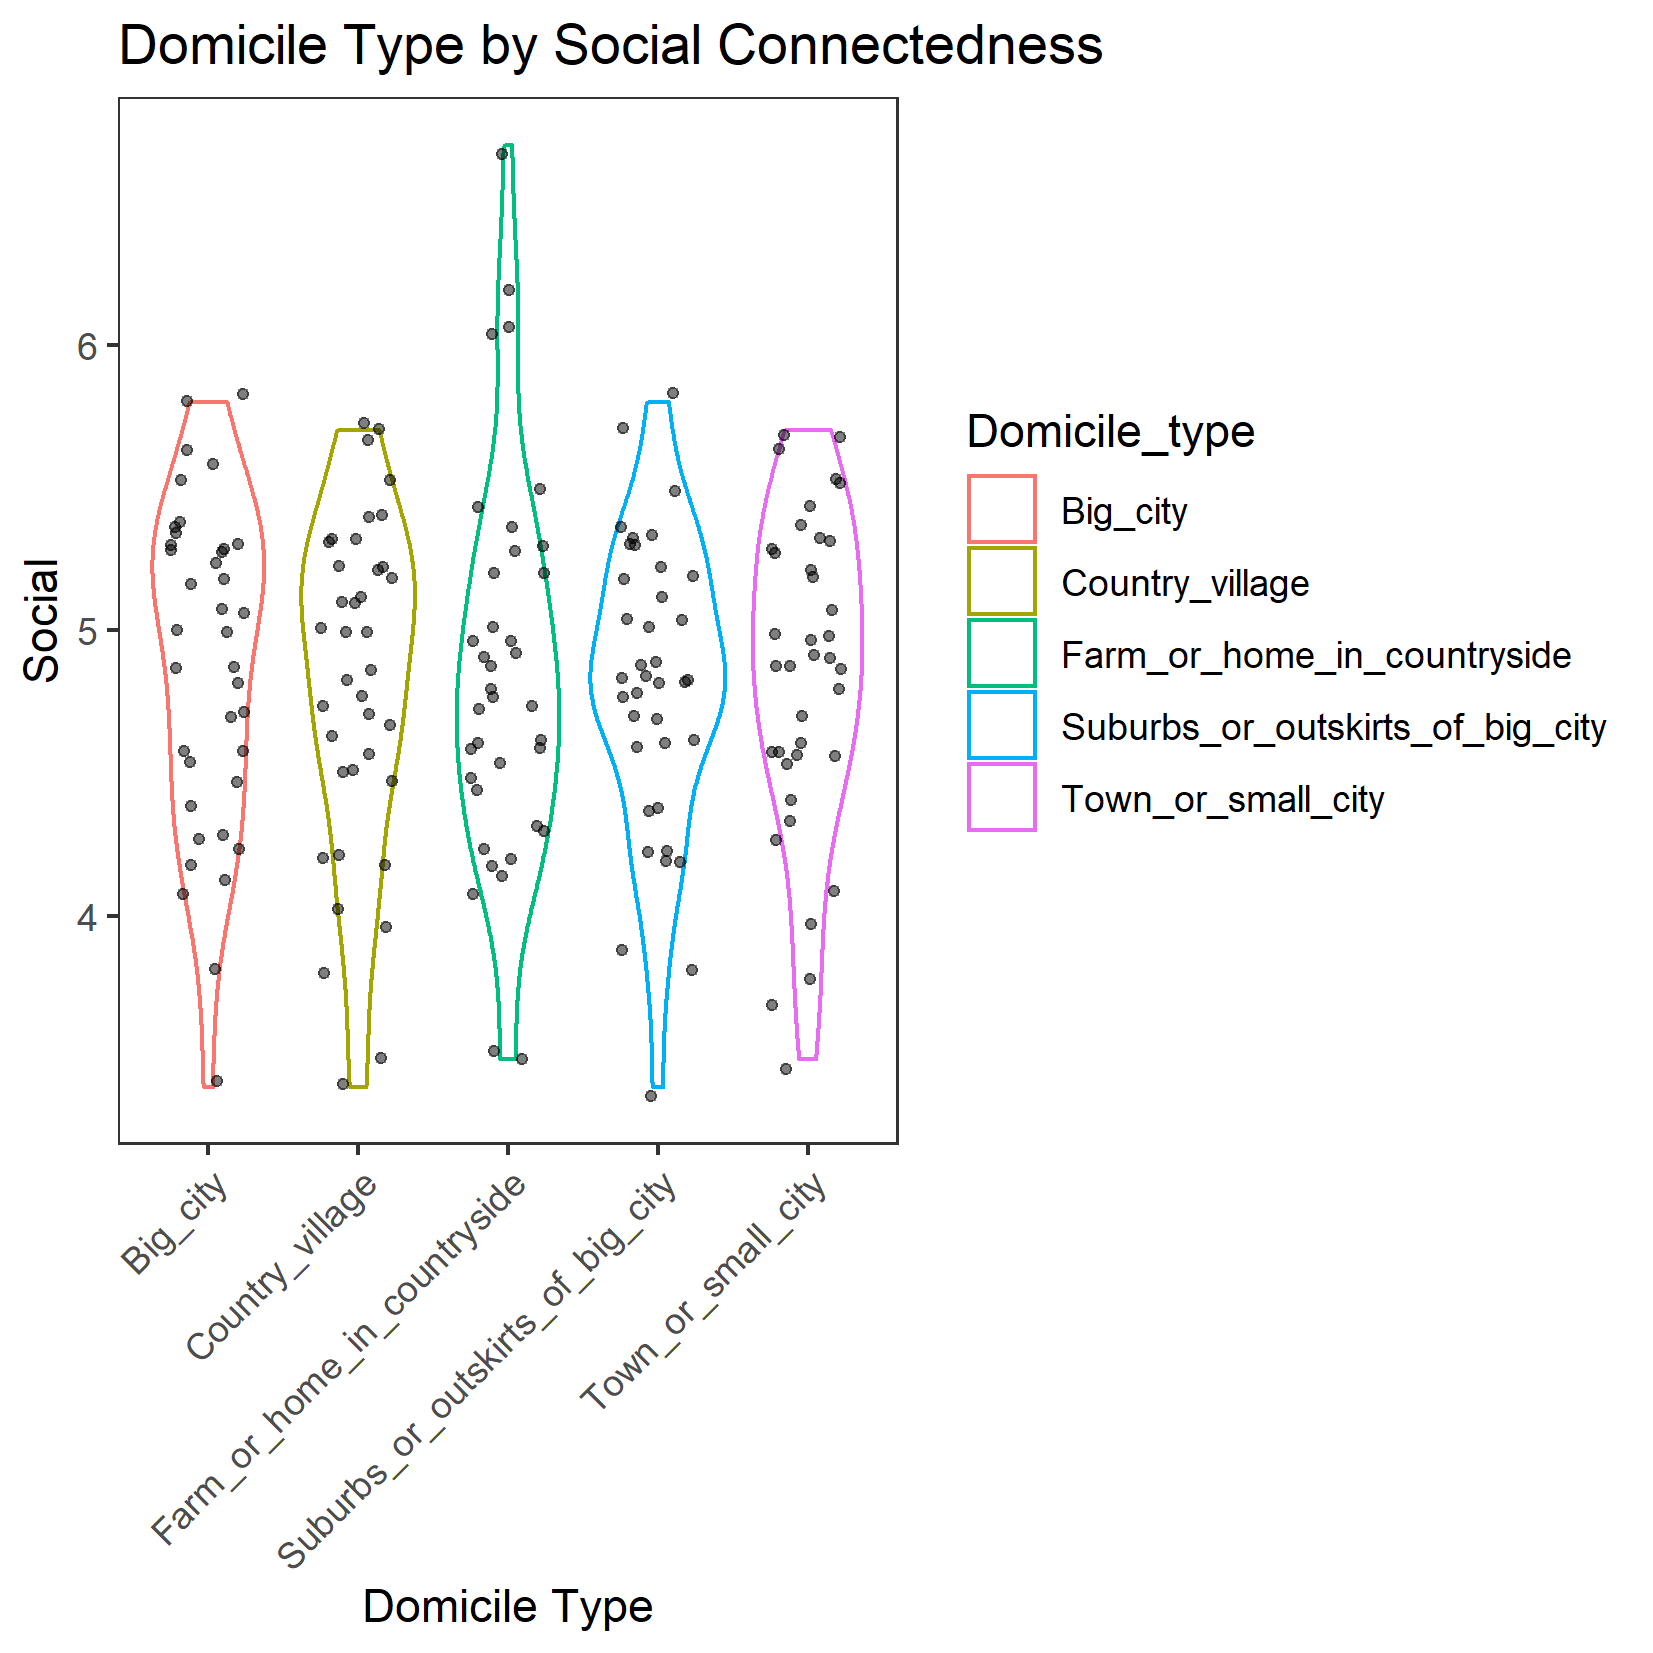
\includegraphics[width=1\linewidth]{C:/Users/annwozniak/Desktop/EEB_Final_Project_Wozniak/Figures/graph_violin_Domicile_by_Social} \caption[Domicile type by social (0-7 scale, never to daily)]{Domicile type by social (0-7 scale, never to daily)}\label{fig:fig.3}
\end{figure}
\end{Schunk}

Is social connectedness significantly correlated to health? When looking
at the relationships among environmental variables, social connectedness
by health, a linear regression analysis and Kruskal-Wallis rank sum test
shows that, social connectedness is significantly correlated to health,
p \textless{} 0.01 for both. Social connectedness is has a positive
relationship to health (Fig. 4), indicating health improves as frequency
of socialization increases.

\begin{Schunk}
\begin{figure}
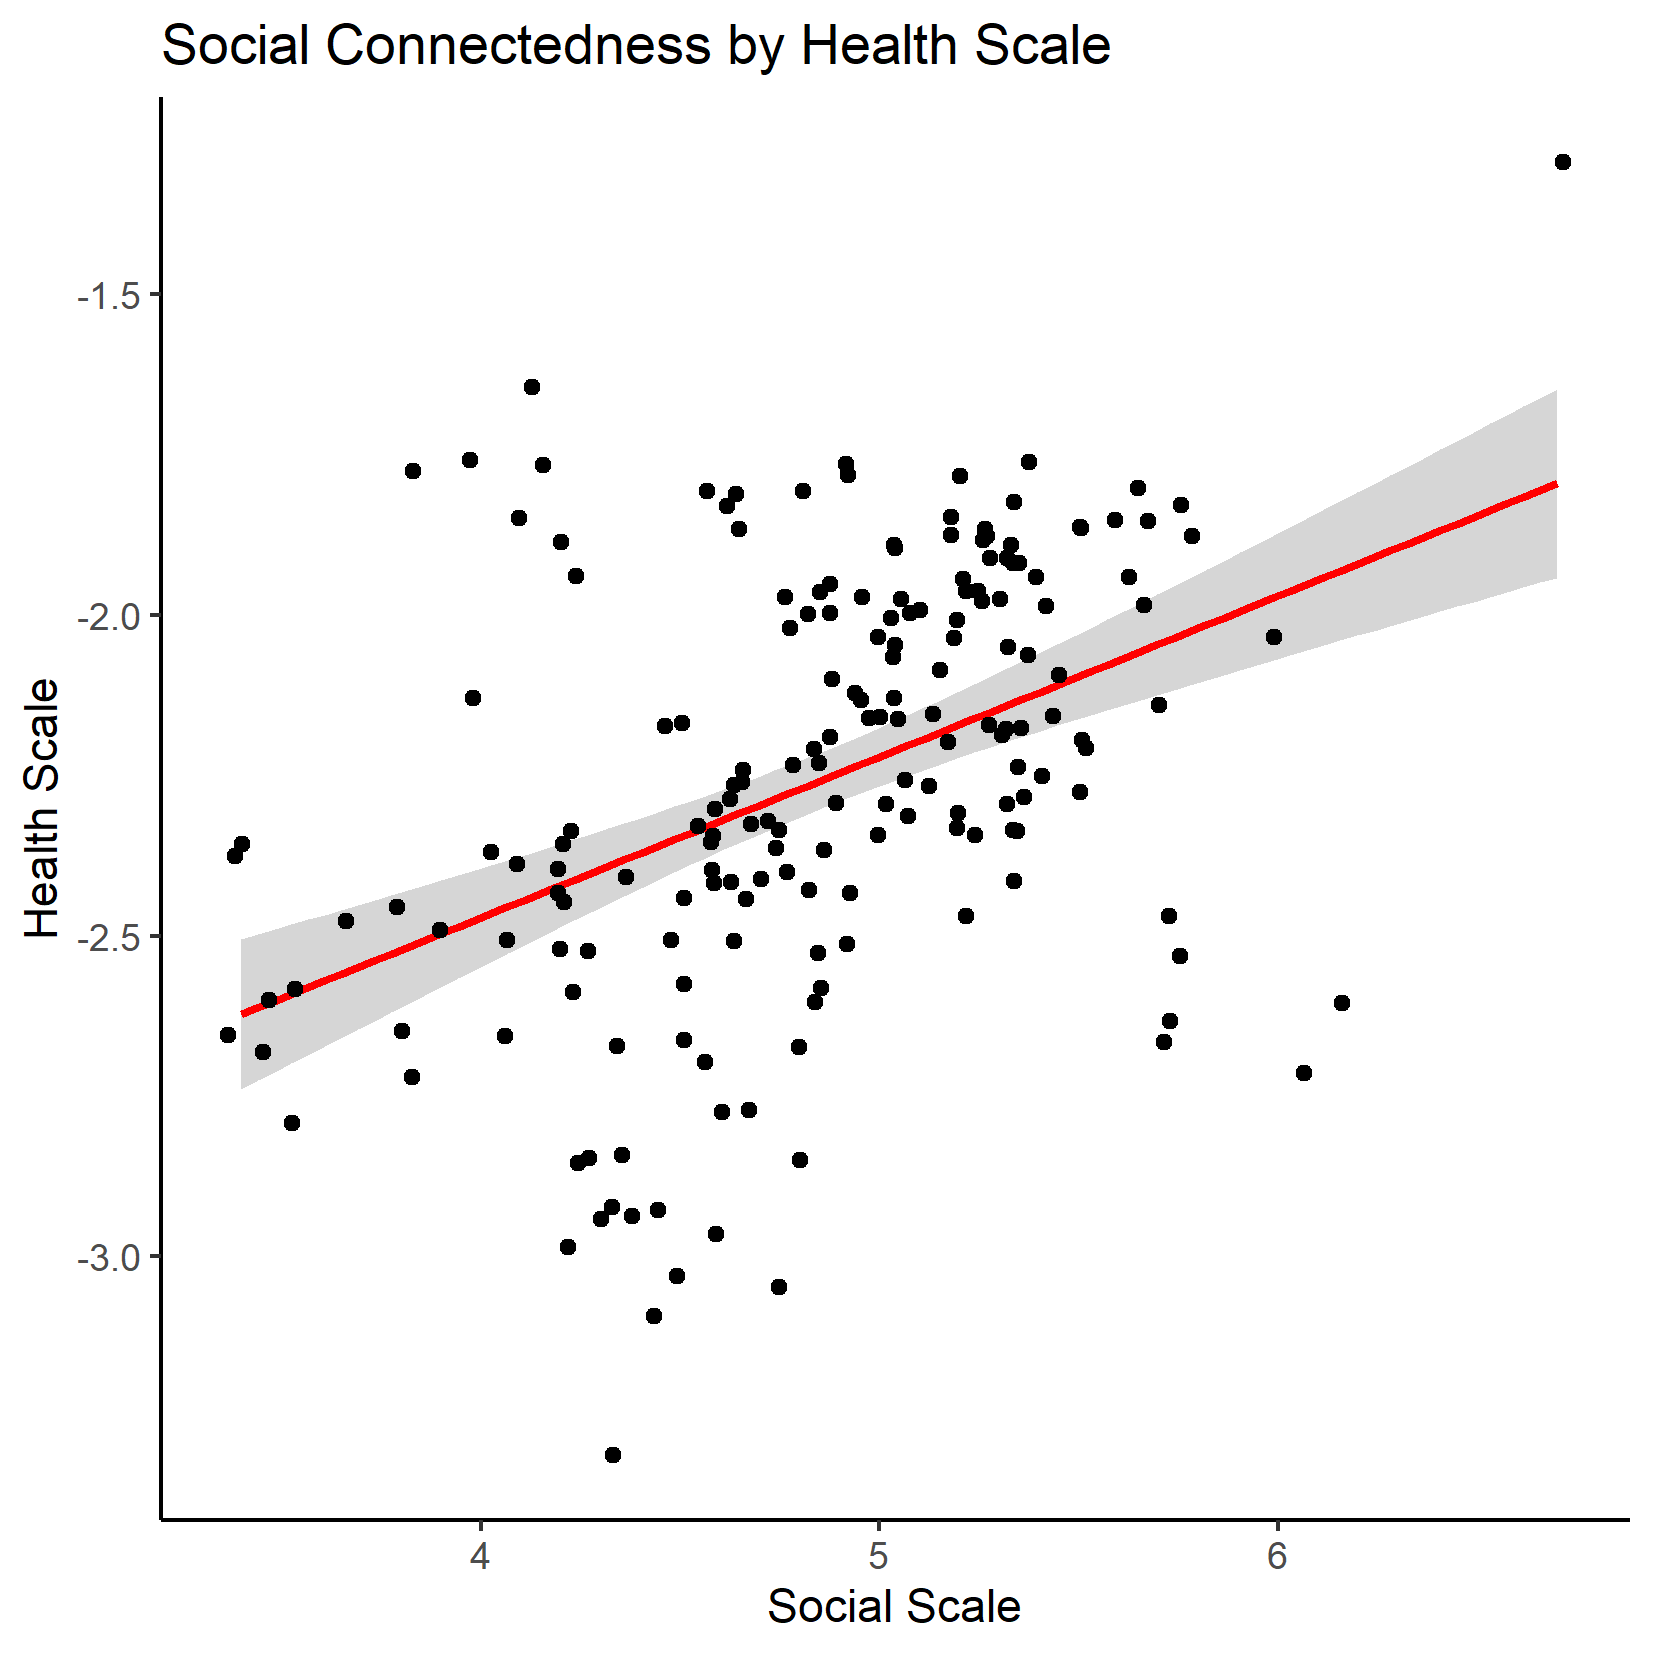
\includegraphics[width=1\linewidth]{C:/Users/annwozniak/Desktop/EEB_Final_Project_Wozniak/Figures/graph_linear_Social_by_Health} \caption[Social connectedness by health linear model]{Social connectedness by health linear model}\label{fig:fig.4}
\end{figure}
\end{Schunk}

Is happiness significantly correlated to health? When looking at the
relationships among environmental variables, happiness by health, a
linear regression analysis and Kruskal-Wallis rank sum test shows that,
happiness is significantly correlated to health, p \textless{} 0.01 for
both. Happiness has a positive relationship to health (Fig. 5),
indicating health improves as happiness increases.

\begin{Schunk}
\begin{figure}
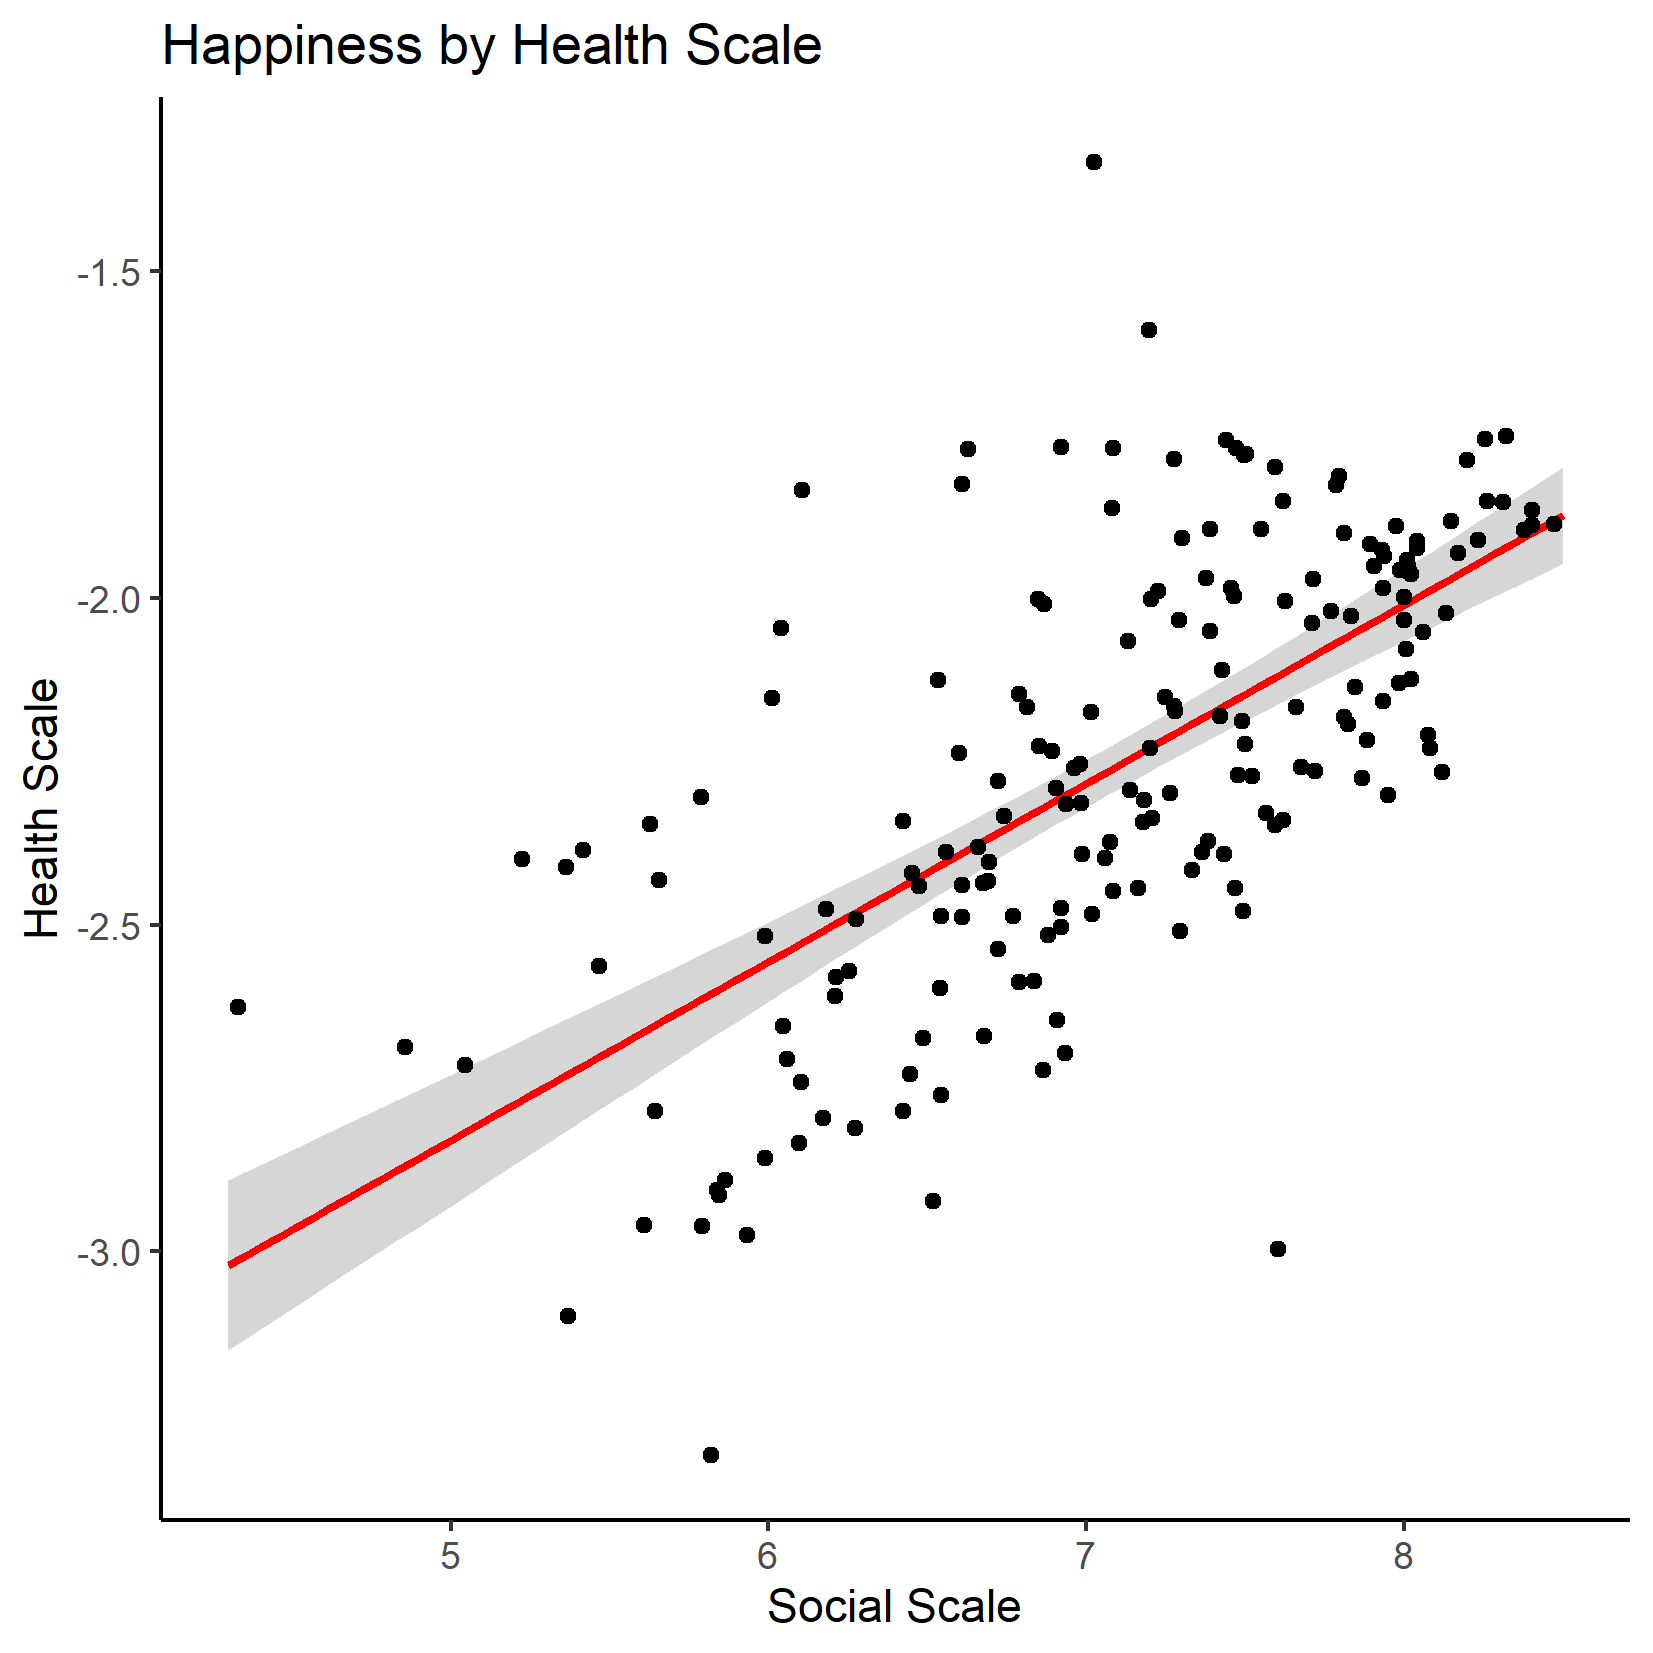
\includegraphics[width=1\linewidth]{C:/Users/annwozniak/Desktop/EEB_Final_Project_Wozniak/Figures/graph_linear_Happy_by_Health} \caption[Happiness by health linear model ]{Happiness by health linear model }\label{fig:fig.5}
\end{figure}
\end{Schunk}

Diversity After removing sites with less than 100 observations, there
were still 146 out of 190 sites with more than 100 observations per site
(Fig. 6).

\begin{Schunk}
\begin{figure}
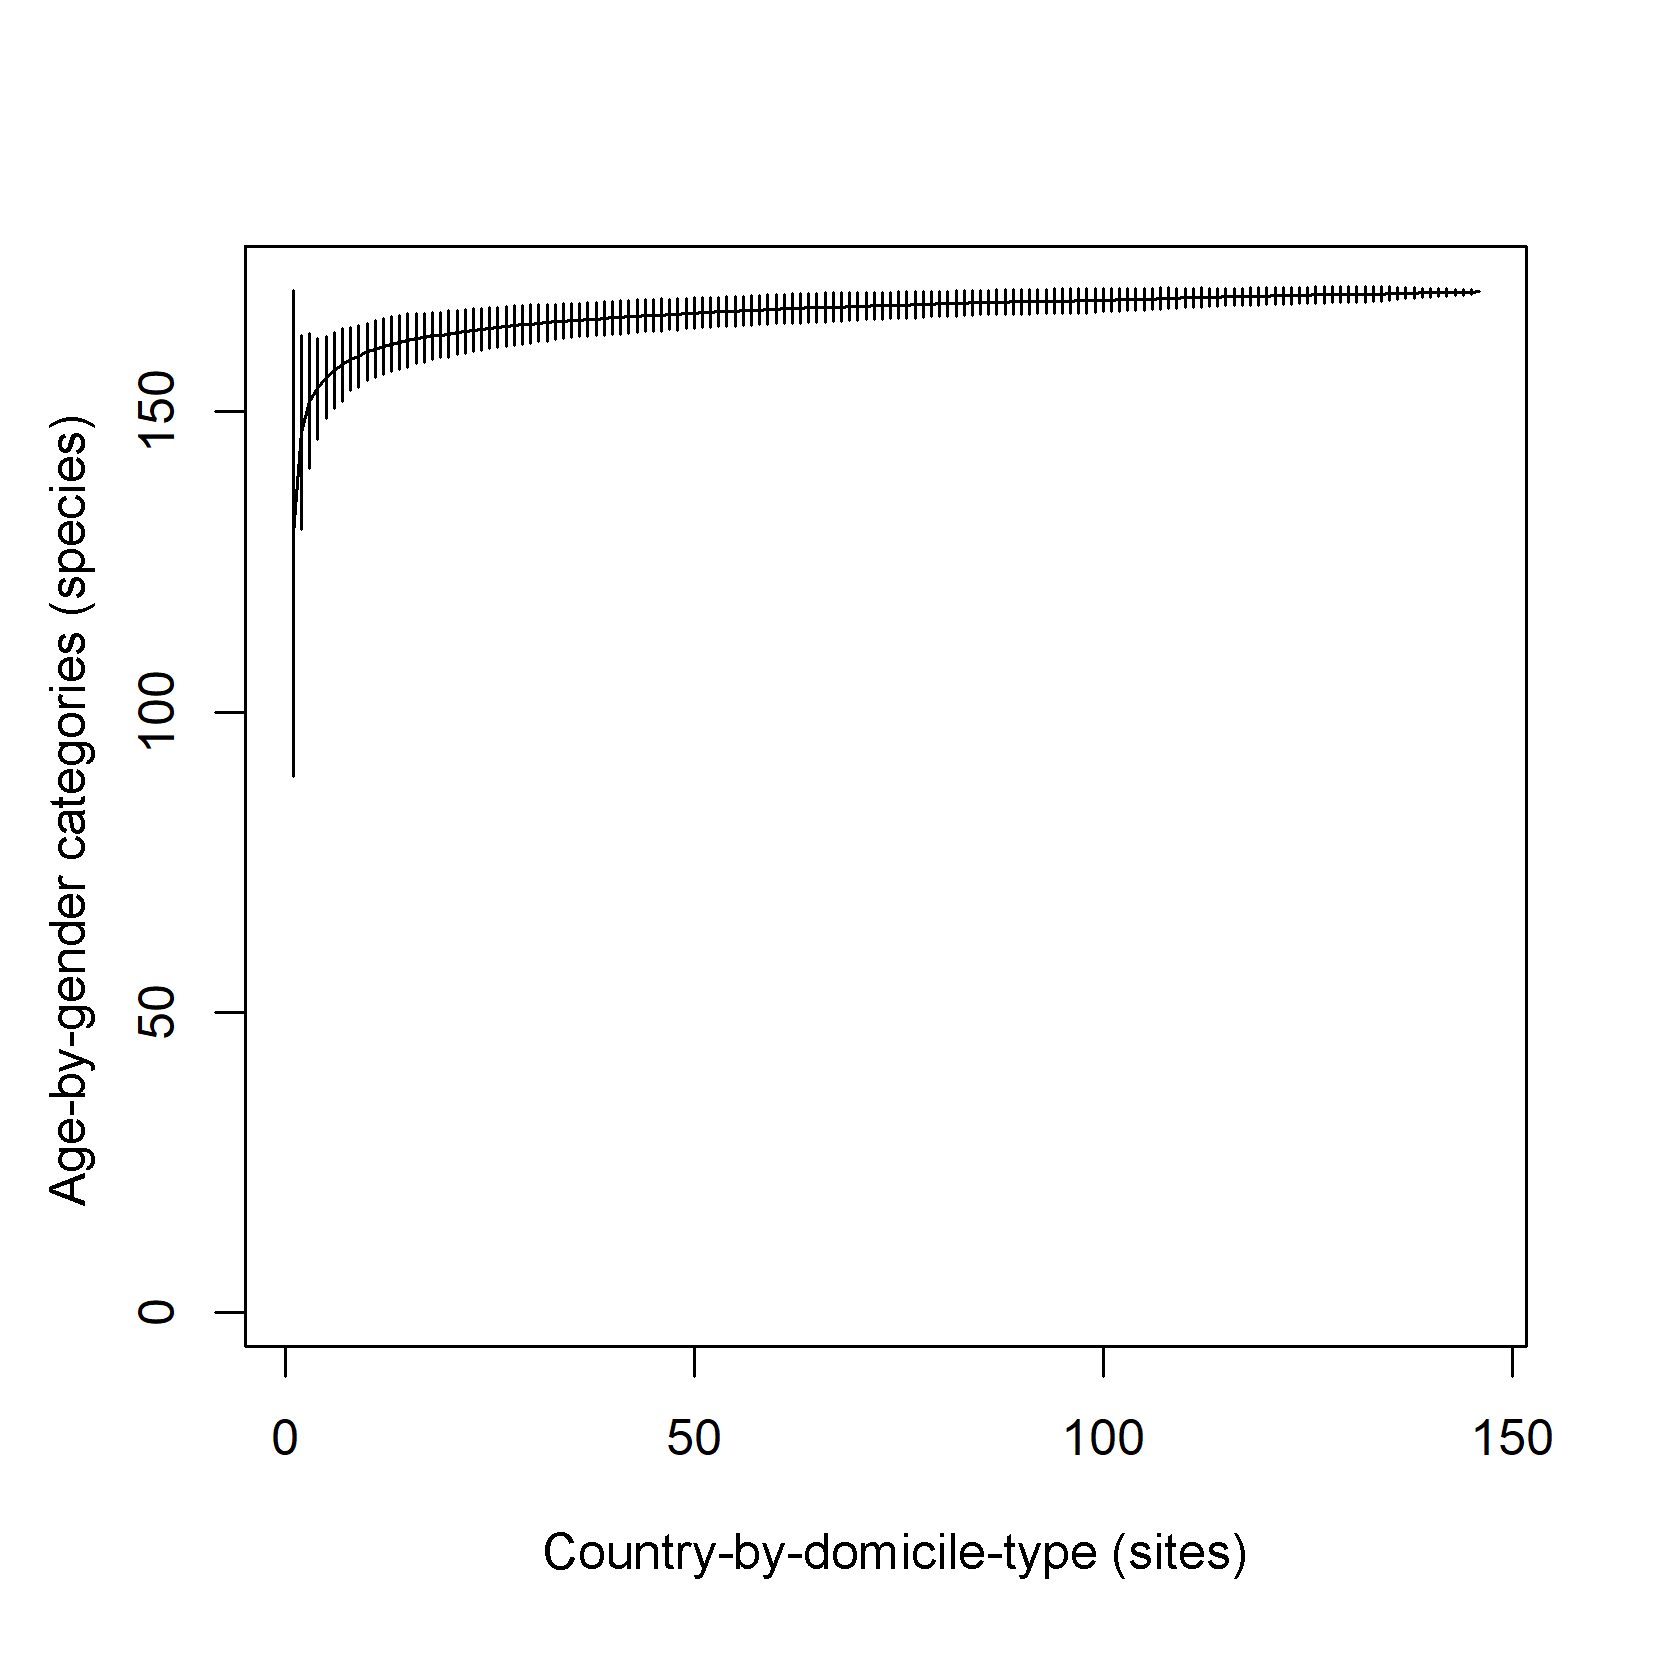
\includegraphics[width=1\linewidth]{C:/Users/annwozniak/Desktop/EEB_Final_Project_Wozniak/Figures/Species-individual_curve2} \caption[Species-Individual Curve Plot]{Species-Individual Curve Plot}\label{fig:fig.6}
\end{figure}
\end{Schunk}

Alpha diversity was measured by species number, Shannon diversity,
effective number of species, and effective number of species, rounded to
the nearest integer. Here, the species are represented as age-by-gender
and alpha diversity simply means abundance or species richness in an
ecosystem or site. Ireland\_farm\_or\_home\_in\_countryside has the
highest number of species at 157 and 5,057 observations.
Turkey\_country\_village has the lowest number of species at 56 and 110
observations. United\_Kingdom\_suburbs\_or\_outskirts\_of\_big\_city has
the highest Shannon diversity at 4.911929 and the highest effective
number of species at 135.90134 (rounded to 136) with 155 species and
2,026 observations. Turkey\_country\_village has the lowest Shannon
diversity at 3.848964 and the lowest effective number of species at
46.94439 (rounded to 47) with 56 species and 110 observations.

What is the relationship between environmental factors and the effective
number of species? A big city has the highest effective number of
species, followed by a town or small city, country or village, suburbs,
and farm or home in countryside respectively (Fig. 7a). The effective
number of species is positively related to happiness and is negatively
related to health (1-5 scale, good to poor) and social connectedness
(Fig. 7b-d).

\begin{Schunk}
\begin{figure}
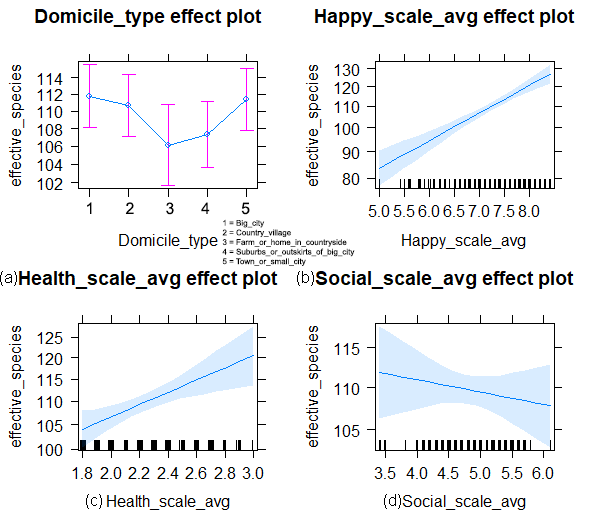
\includegraphics[width=1\linewidth]{C:/Users/annwozniak/Desktop/EEB_Final_Project_Wozniak/Figures/Effective_number_of_species_by_metadata2} \caption[(a) Effective number of species by domicile type,  (b) Effective number of species by happiness (0-10 scale, unhappy to happy), (c) Effective number of species by health (1-5 scale, good to poor), and (d) Effective number of species by social connectedness (0-7 scale, never to daily)]{(a) Effective number of species by domicile type,  (b) Effective number of species by happiness (0-10 scale, unhappy to happy), (c) Effective number of species by health (1-5 scale, good to poor), and (d) Effective number of species by social connectedness (0-7 scale, never to daily)}\label{fig:fig.7}
\end{figure}
\end{Schunk}

Beta diversity was measured by comparing diversity of species
(age-by-gender) across different ecosystems or sites. Here, sites are
represented as country-by-domicile type. Diversity across sites were
measured using Bray-Curtis (Fig. 8) and the binary version of Jaccard
(Fig. 9) Non-metric Multi-dimensional Scaling (NMDS) ordinal plots. Both
methods yielded no convergence, even when increasing from k = 2 to 3
dimensions. Turkey and Romania country villages appear to be most
distant from the others in terms of their diversity (age-by-gender).

\begin{Schunk}
\begin{figure}
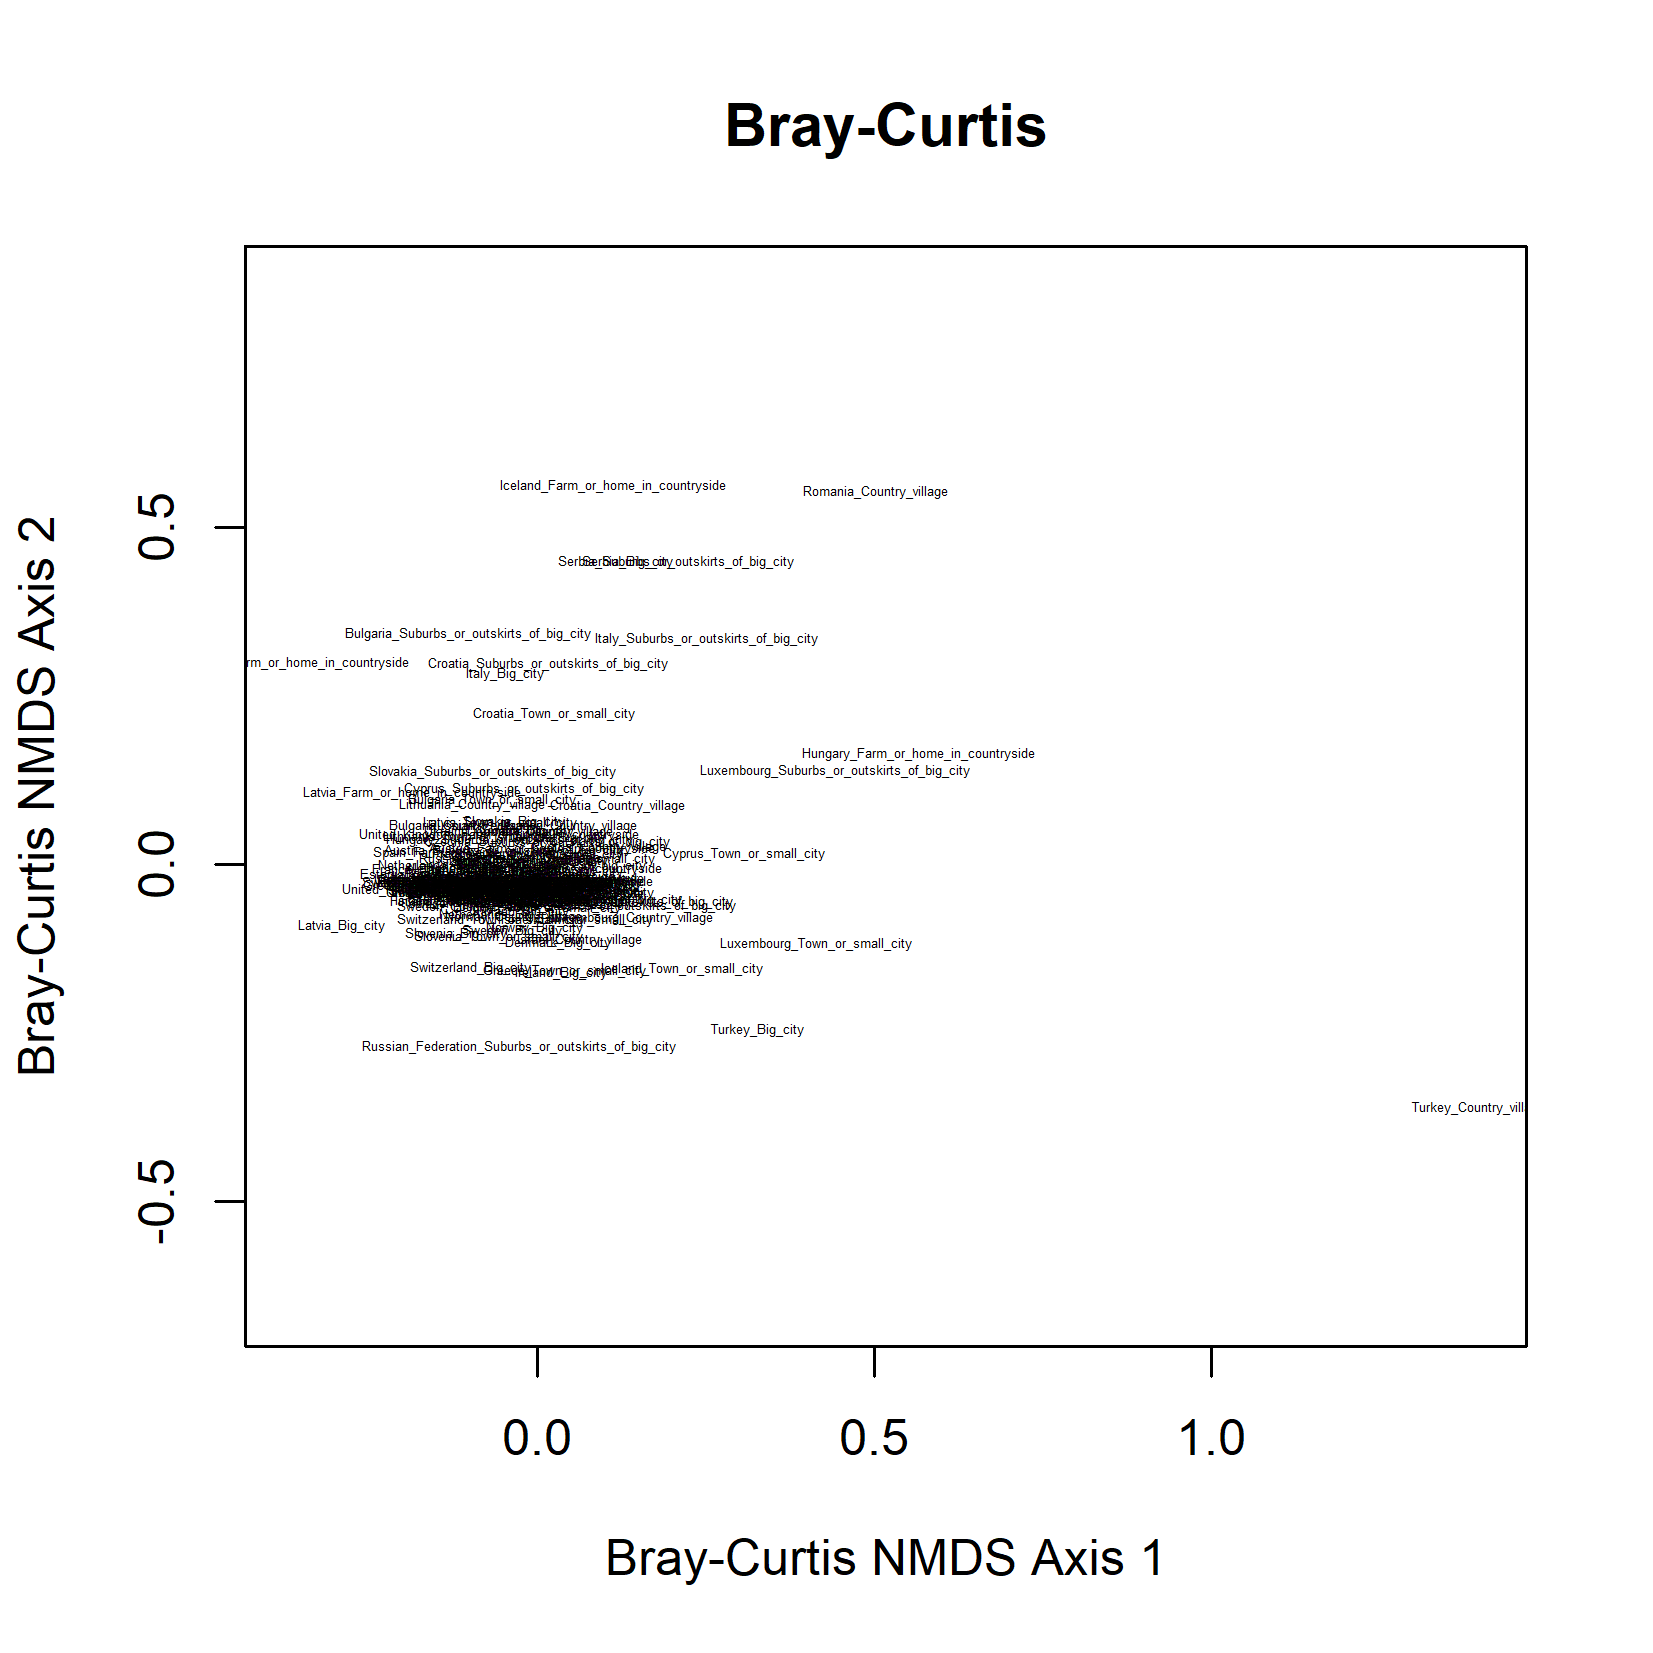
\includegraphics[width=1\linewidth]{C:/Users/annwozniak/Desktop/EEB_Final_Project_Wozniak/Figures/Bray-Curtis} \caption[Bray-Curtis NMDS]{Bray-Curtis NMDS}\label{fig:fig.8}
\end{figure}
\end{Schunk}

\begin{Schunk}
\begin{figure}
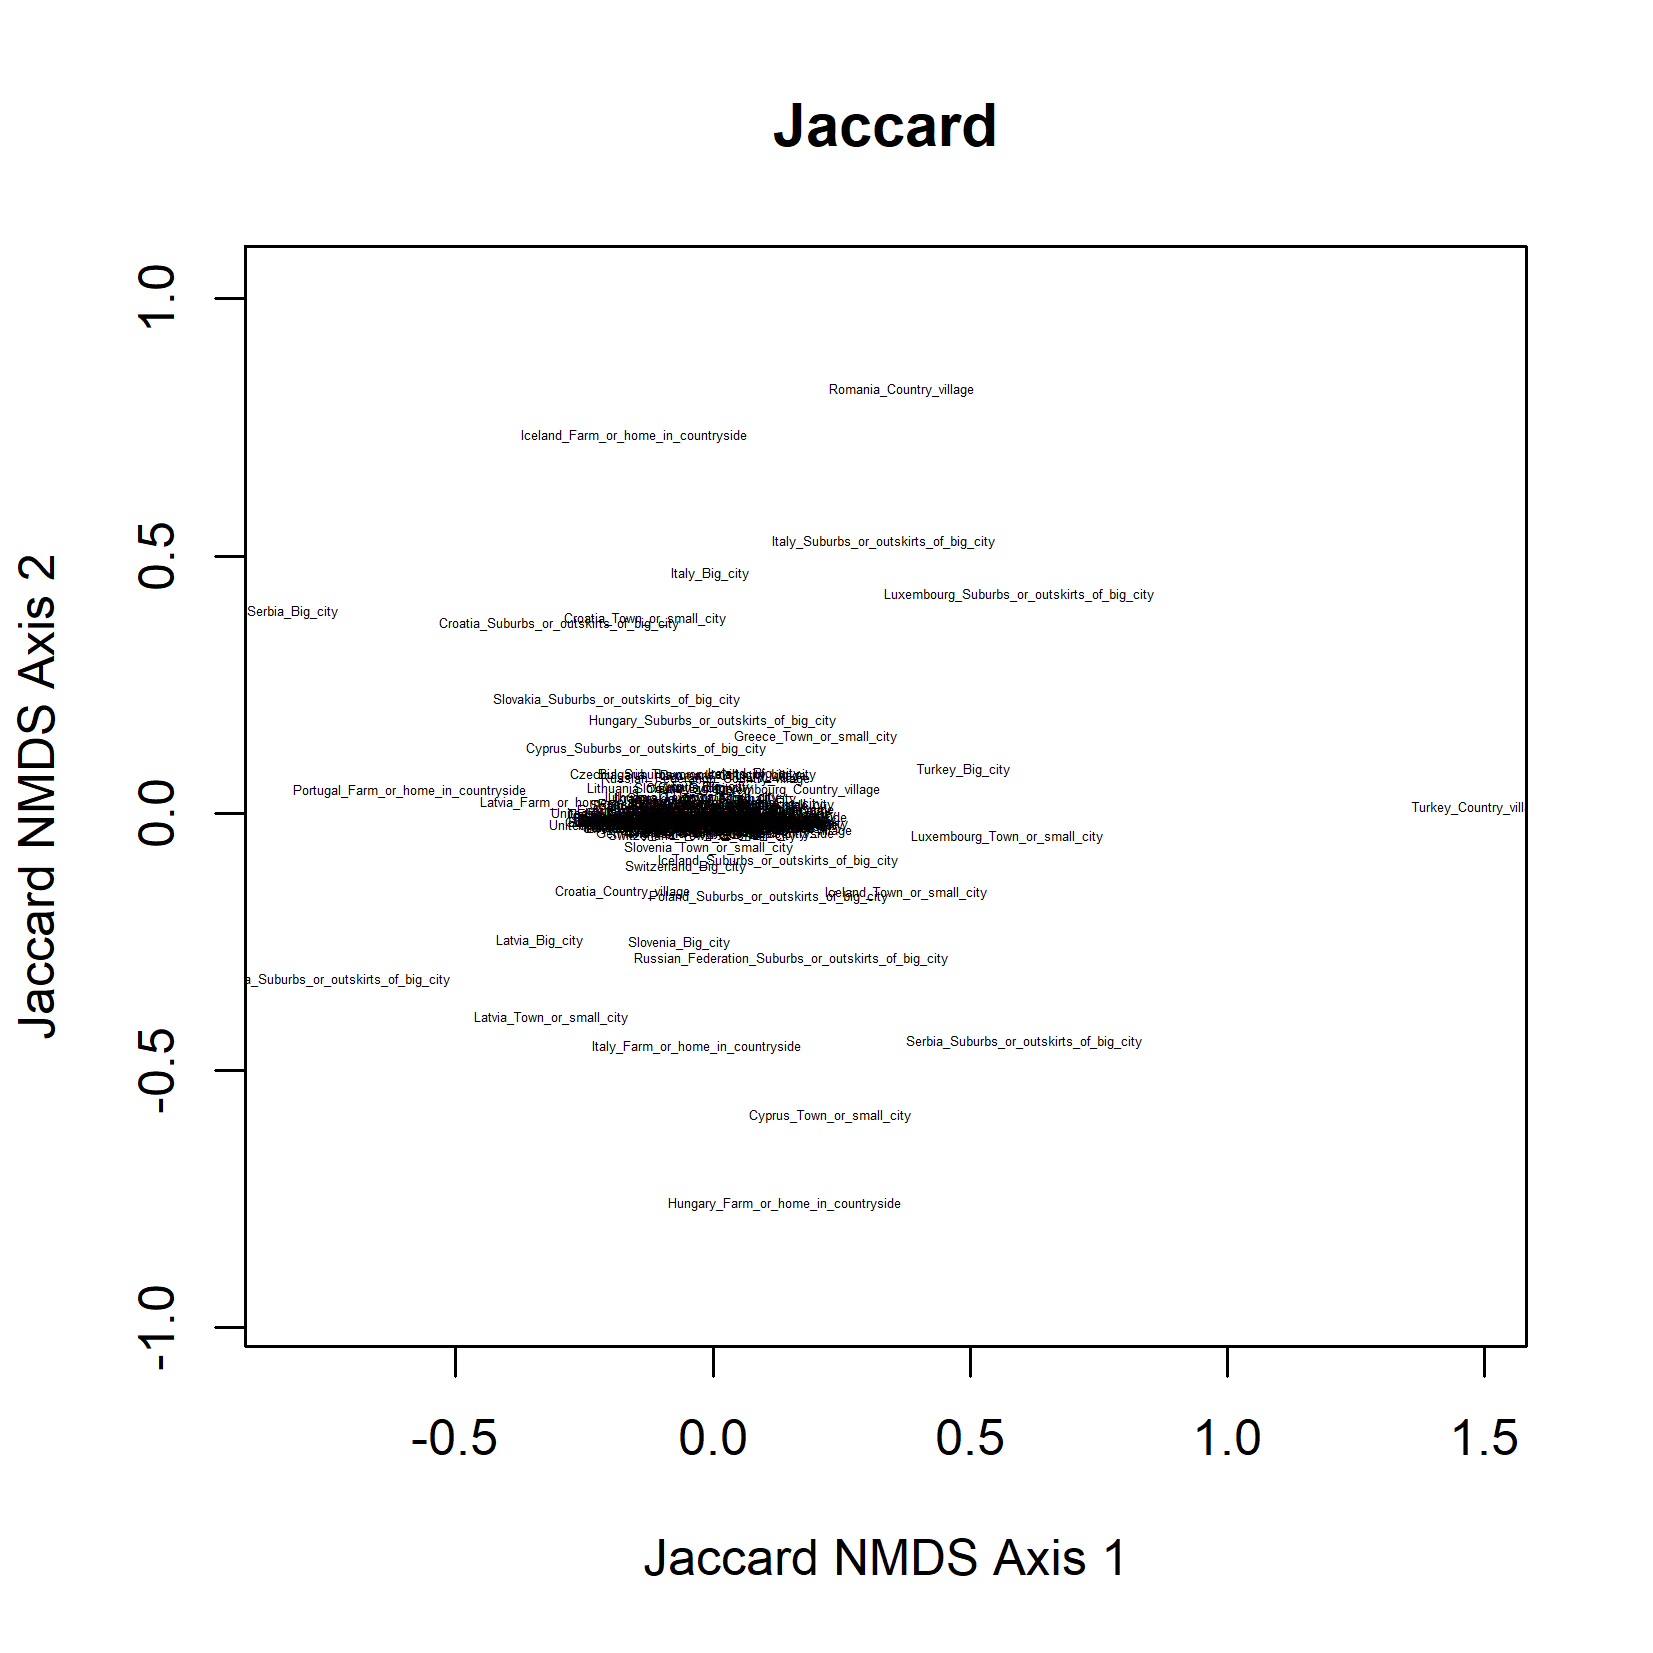
\includegraphics[width=1\linewidth]{C:/Users/annwozniak/Desktop/EEB_Final_Project_Wozniak/Figures/Jaccard} \caption[Jaccard NMDS]{Jaccard NMDS}\label{fig:fig.9}
\end{figure}
\end{Schunk}

Is beta diversity significantly correlated to country or domicile type?
Using a PERMANOVA test shows that, both country and domicile type are
significantly correlated to beta diversity, p \textless{} 0.001 and with
country having a larger R-squared value of 0.33957 compared to a
R-squared value of 0.05230 for domicile type.

Is there a correlation between ``species'' and happiness across sites?
There is a significant correlation between ``species'' and happiness
across sites, mantel statistic r = 0.2346, p = 0.001.

Is there a correlation between ``species'' and health across sites?
There is a significant correlation between ``species'' and health across
sites, mantel statistic r = 0.09944, p = 0.021.

Is there a correlation between ``species'' and social connectedness
across sites? There is not a significant correlation between ``species''
and social connectedness across sites, mantel statistic r = 0.08752, p =
0.06.

\hypertarget{discussion}{%
\subsection{Discussion}\label{discussion}}

This study indicates that using a human community framework to determine
if domicile type is correlated to health, happiness or social
connectedness shows that they are not significantly correlated while
happiness and social connectedness are significantly correlated to
health. Previous analysis utilizing SPSS indicated a significant
correlation between each variable at an individual level. When
reproduced in R at the individual level, this holds true. The only
discrepancy between the two scales were with domicile type. Perhaps the
distribution of ``species'' across domicile types accounts for the
discrepancies. A cross comparison of the same number of ``species'' in
each category might have a different outcome. Further analysis needs to
be done to understand the discrepancies between the community and
individual scale.

When looking at the relationships among environmental variables, social
connectedness and happiness are significantly correlated to health, p
\textless{} 0.01 with a positive relationships. In other words, health
increases as happiness and social connectedness increase. These findings
match research and my hypothesis. A community scale analysis may be an
effective tool when linking social connectedness and happiness to
health.

Analysis of alpha and beta diversity followed my expectations in that
Shannon diversity and effective number of species were highest in
cities. Not surprisingly, the effective number of species is positively
related to happiness; meaning that the more diverse a human
society---here analyzed as an ecosystem, the greater the happiness.
Contrary to my hypothesis, effective number of species is negatively
related to social connectedness and health. In other words, social
connections and health go down as diversity, measured in age-by-gender
categories, increases. Both country and domicile type are significantly
correlated to beta diversity, with country having a larger impact. There
is a significant correlation between community composition and happiness
as well as community composition and health across sites. Similar to
findings of effective number of species and social connectedness,
community composition and social connectedness are not a significantly
correlated across sites. Perhaps this has more to do with how
cooperation within and between groups are linked by similarities in age
and gender, rather than differences, and that social connections are not
important drivers when analyzing human societies in a community ecology
framework.

\hypertarget{citation-of-data}{%
\subsection{Citation of Data}\label{citation-of-data}}

ESS Round 9: European Social Survey Round 9 Data (2018). Data file
edition 2.0. NSD - Norwegian Centre for Research Data, Norway -- Data
Archive and distributor of ESS data for ESS ERIC.
\url{doi:10.21338/NSD-ESS9-2018}.

ESS Round 8: European Social Survey Round 8 Data (2016). Data file
edition 2.1. NSD - Norwegian Centre for Research Data, Norway -- Data
Archive and distributor of ESS data for ESS ERIC.
\url{doi:10.21338/NSD-ESS8-2016}.

ESS Round 7: European Social Survey Round 7 Data (2014). Data file
edition 2.2. NSD - Norwegian Centre for Research Data, Norway -- Data
Archive and distributor of ESS data for ESS ERIC.
\url{doi:10.21338/NSD-ESS7-2014}.

ESS Round 6: European Social Survey Round 6 Data (2012). Data file
edition 2.4. NSD - Norwegian Centre for Research Data, Norway -- Data
Archive and distributor of ESS data for ESS ERIC.
\url{doi:10.21338/NSD-ESS6-2012}.

ESS Round 5: European Social Survey Round 5 Data (2010). Data file
edition 3.4. NSD - Norwegian Centre for Research Data, Norway -- Data
Archive and distributor of ESS data for ESS ERIC.
\url{doi:10.21338/NSD-ESS5-2010}.

ESS Round 4: European Social Survey Round 4 Data (2008). Data file
edition 4.5. NSD - Norwegian Centre for Research Data, Norway -- Data
Archive and distributor of ESS data for ESS ERIC.
\url{doi:10.21338/NSD-ESS4-2008}.

ESS Round 3: European Social Survey Round 3 Data (2006). Data file
edition 3.7. NSD - Norwegian Centre for Research Data, Norway -- Data
Archive and distributor of ESS data for ESS ERIC.
\url{doi:10.21338/NSD-ESS3-2006}.

ESS Round 2: European Social Survey Round 2 Data (2004). Data file
edition 3.6. NSD - Norwegian Centre for Research Data, Norway -- Data
Archive and distributor of ESS data for ESS ERIC.
\url{doi:10.21338/NSD-ESS2-2004}.

ESS Round 1: European Social Survey Round 1 Data (2002). Data file
edition 6.6. NSD - Norwegian Centre for Research Data, Norway -- Data
Archive and distributor of ESS data for ESS ERIC.
\url{doi:10.21338/NSD-ESS1-2002}.

\bibliography{Peer-Article-Wozniak-2020.bib}

\address{%
Ann Wozniak AIA, NCARB, LEED AP BD+C, NCIDQ\\
Boise State University, Ecology, Evolution, and Behavior\\%
1910 W. University Drive\\ Boise, ID, 83725\\
%
\url{https://journal.r-project.org}%
\\\textit{ORCiD: \href{https://orcid.org/0000-0002-2655-7283}{0000-0002-2655-7283}}%
\\\href{mailto:annwozniak@boisestate.edu}{\nolinkurl{annwozniak@boisestate.edu}}
}
